\begin{abstract}
Edge servers that act on a monitored process need an estimate that is correct, not merely recent. In
satellite-ground integrated networks (SAGIN), satellite handover and shadowing interrupt links for long enough that the
monitored process can change state several times, so the age of incorrect information (AoII) is the appropriate
measure of estimation quality. This paper formulates the robust, network-level AoII minimization problem VANGUARD, in
which update rates, serving-node association, and bandwidth are chosen jointly to minimize the worst-case time-average
AoII over a set of disruption scenarios, and solves it with SENTINEL, a distributed hybrid quantum-classical procedure.
A renewal-interval decomposition turns the history-dependent AoII into a closed-form cost per inter-delivery
interval. The minimax over scenarios is dualized into scenario weights updated by a classical outer loop, so that each
satellite-ground domain solves a linear assignment subproblem encoded as a compact quadratic unconstrained binary
optimization (QUBO) whose one-hot structure is enforced by XY mixers rather than penalties; the domains are coordinated
through the sharing form of ADMM, and every returned schedule is certified by its exact worst-case AoII. The
evaluation uses Starlink ephemerides, the 3GPP TR 38.811 non-terrestrial channel, and acknowledgement feedback for
all policies, with an exact integer-programming reference and paired tests over 30 to 60 seeds. The
certificate held in 98.7\% of orchestration epochs under real passes; the robust schedule's certified worst case is 2
to 7\% below that of the nominal schedule at no measurable cost in realized AoII, and SENTINEL combined with a
state-aware transmission trigger comes within 10 to 20\% of the best per-slot heuristic while retaining the
certificate. Without failure feedback every policy degrades by an order of magnitude and the hybrid is 25 to 30\%
better than the per-slot heuristic at the larger network sizes. The quantum step is exact through 25 UEs in simulation with four to five times
fewer qubits than a direct epigraph encoding, and thirteen domains of 8 to 38 qubits sampled on two IBM Heron
processors all decoded to the exact optimum, with the fraction of usable shots falling from 86\% to 2.6\% over that
range. At these sizes the quantum sampler is correct but not a better optimizer than greedy association, and we report
this limit together with the scale at which it would matter.
\end{abstract}

\begin{IEEEkeywords}
6G, age of incorrect information (AoII), alternating direction method of multipliers (ADMM), mission-critical edge
computing, non-terrestrial networks, quantum approximate optimization algorithm (QAOA), remote estimation, robust
optimization, satellite-ground integrated network (SAGIN)
\end{IEEEkeywords}

\IEEEpeerreviewmaketitle

%=======================================================================
\section{Introduction}
%=======================================================================

Sixth-generation networks are expected to place decision-making at the edge~\cite{Saad2020}: an edge server that
monitors a hazard indicator, the integrity of a structure, or the position of an asset must act on its own estimate of
that process, often without a human in the loop. What matters to such a server is whether its estimate is still
correct. Terrestrial mobile edge computing provides capacity and low delay where ground infrastructure exists, which is
often not where monitoring is most needed, and satellite links extend coverage to the remaining regions at the price of
intermittent connectivity~\cite{Giordani2021}. The combination, a satellite-ground integrated network (SAGIN), is the
setting of this paper.

Satellite links fail in ways that terrestrial links rarely do. A low-earth-orbit satellite sets and hands the user over
to the next one every few minutes; buildings and foliage block the line of sight for the length of a pass; shadow
fading in the non-line-of-sight state exceeds ten decibels~\cite{TR38811}. During any of these interruptions the
monitored process keeps evolving, and by the time the link is restored the edge estimate may be wrong by several
states rather than simply old. The age of information (AoI)~\cite{Kaul2012, Yates2021} measures only elapsed time and
cannot tell these two situations apart. The age of incorrect information (AoII)~\cite{Maatouk2020, Maatouk2023} can:
it is zero while the estimate is correct and grows with the duration and the magnitude of a mismatch. AoII has been
analyzed mainly for one source and one monitor on a point-to-point channel. Carrying it to a network of edge nodes,
satellites, and base stations raises two difficulties. The metric depends on the whole trajectory of the source since
the estimate was last correct, so it does not fit the per-slot cost structure of the assignment problems used for
SAGIN resource allocation. And the duration of a mismatch is governed by outages whose length is uncertain, so the
allocation must be judged by its worst case over plausible disruptions, not by its average.

We treat the problem as robust combinatorial optimization. The first step is a renewal-interval decomposition: a source
that evolves as a Markov chain with known transition matrix accumulates, between two deliveries, an expected AoII that
depends only on the length of the interval, and this quantity can be tabulated offline. The channel then enters the
objective through a single number per scenario, the inter-delivery interval, and the resulting robust scheduling
problem, VANGUARD, is a minimax assignment problem over binary variables. The second step concerns how such a problem
can be given to a quantum solver. A direct encoding of the minimax, with an epigraph variable and one slack register
per scenario, needs three to four auxiliary qubits for every decision qubit and a penalty landscape in which classical
and quantum local search alike fail to find a feasible point; we document this failure in Section~VI. SENTINEL instead
dualizes the minimax into scenario weights that a classical outer loop updates by exponentiated gradient, so that each
inner subproblem has a linear objective and is encoded as a compact QUBO over the decision variables and a few
capacity-slack bits. The one-hot constraint of each user is enforced by the XY mixer of the quantum circuit rather
than by a penalty~\cite{Hadfield2019}, which keeps every sample a valid assignment. The network is partitioned into
satellite-ground domains that are coordinated by the sharing form of ADMM~\cite{Boyd2011}, and each assembled schedule
is evaluated exactly under every scenario, so the reported worst case is a certificate that does not rest on the
solver's optimality.

The third step is an evaluation that a reader can trust. Satellite passes are propagated from a Starlink
two-line-element snapshot with SGP4~\cite{Vallado2006}; the large-scale channel follows the suburban tables of
3GPP TR 38.811~\cite{TR38811}, including the elevation-dependent line-of-sight probability and clutter loss; every
policy, including the baselines, receives acknowledgement feedback and may abandon a link that has failed for a fixed
time; an integer linear program solved to optimality provides the reference for every solver; and all policies run on
the same random episodes, so that comparisons are paired and are reported with signed-rank tests. The quantum step is
run on two IBM Heron processors as well as in simulation.

The results support a modest and precisely stated set of claims. Under real passes the worst-case certificate held in
98.7\% of orchestration epochs, and its violations are non-line-of-sight passes whose clutter loss exceeds the
scenario set. The robust schedule's certificate is 2 to 7\% lower than that of its nominal counterpart in 67 to 100\%
of seeds, while the two are statistically indistinguishable in realized AoII, with and without failure feedback; the
value of the scenario set is the guarantee, not a lower average. A per-slot policy that transmits whenever its
observed AoII is positive is the strongest heuristic when feedback is available, and we show that it coincides with
the Whittle-index scheduler of the restless-bandit literature~\cite{Whittle1988, Kadota2018} at the bandwidths of this
study; SENTINEL combined with the same trigger comes within 10 to 20\% of it while keeping the certificate, and is 25 to
30\% better than it at 15 to 20 users when feedback is removed. The compact formulation is exact through 25 users and
within 12\% at 50 with four to five times fewer qubits than the epigraph encoding; its limit at 75 to 100 users is the
coordination of shared satellites, not the inner solver. On hardware, thirteen domains of 8 to 38 qubits sampled on
\texttt{ibm\_kingston} and \texttt{ibm\_fez} all decoded to the exact optimum, with the fraction of usable shots
decreasing from 86\% to 2.6\% as the circuits grew; a trained proximal-policy-optimization agent, included because
learning-based baselines are expected, matches the nominal schedule at five users and falls behind as its action
space grows. On every instance that fits a current device, greedy association is already optimal, so the quantum step
is a correct, hardware-runnable constrained sampler and not yet a better optimizer; the instances on which greedy
loses need one to two hundred qubits per domain.

The contributions of this paper are the following.
\begin{itemize}[leftmargin=13pt]
\item The robust scheduling problem VANGUARD, which minimizes the worst-case time-average AoII of a network of
monitored edge nodes over a scenario set of satellite shadowing and handover disruptions, jointly over update rates,
association, and bandwidth, subject to capacity, visibility, rate, and AoII-budget constraints.
\item A renewal-interval decomposition that expresses the expected AoII accumulated between deliveries in closed form
as a function of the interval length and the source's transition matrix, verified against Monte Carlo simulation to
within one percent, which reconciles the history dependence of AoII with binary-variable optimization.
\item SENTINEL, a distributed hybrid procedure in which the minimax is dualized into classically updated scenario
weights, each domain's subproblem is a compact QUBO with XY-mixer-enforced one-hot structure, candidate pruning
removes dominated combinations without changing the optimum, and the sharing form of ADMM with a warm start and a
cost-scaled penalty coordinates the domains; together with a certificate of the worst-case AoII of every schedule.
\item An evaluation under Starlink ephemerides and the TR 38.811 channel, against an exact integer-programming
reference, with paired statistics over 30 to 60 seeds, baselines that include the Whittle-index scheduler and a
trained learning agent, an ablation of failure feedback, sensitivity to the scenario set and to bandwidth, and runs of
the quantum step on two superconducting processors, with the scale limit of the quantum step stated explicitly.
\end{itemize}

The remainder of the paper is organized as follows. Section~II reviews related work. Section~III presents the system
model: the channel and satellite geometry, the monitored sources, the disruption scenarios, the renewal-interval
decomposition, the binary decision model, and the orchestration architecture. Section~IV formulates VANGUARD and its
binary reformulations. Section~V develops the dualized compact QUBO, the XY-mixer QAOA, and the ADMM coordination.
Section~VI reports the evaluation, and Section~VII concludes.

%=======================================================================
\section{State of the Art}
%=======================================================================

The paper touches five bodies of work: satellite-ground integrated edge computing, information freshness and
correctness, robust resource allocation, learning-based scheduling, and quantum-assisted combinatorial optimization.
We take them in turn and then state the gap.

\subsubsection{Satellite-Ground Integrated Edge Computing}
Mobile edge computing~\cite{Mao2017} has been extended beyond terrestrial coverage by placing edge servers on
satellites and base stations~\cite{Liu2018, Kato2019, Zhang2019}. The literature is dominated by task offloading
under deterministic or average channel assumptions~\cite{Cheng2019, Zhou2021}, with the completion delay of a task as
the objective. The correctness of what the server believes about the monitored process has not been the quantity
optimized. On the channel side, the 3GPP study on non-terrestrial networks~\cite{TR38811} provides
elevation-dependent line-of-sight probabilities, clutter losses, and shadow-fading statistics for several
environments, and the SGP4 propagator with public two-line elements~\cite{Vallado2006} gives pass geometry for any
constellation; most SAGIN evaluations use neither, and we found that the choice matters, because with real passes the
dominant disruptions are handovers and non-line-of-sight passes rather than coverage gaps.

\subsubsection{Age of Information and Age of Incorrect Information}
AoI has been studied extensively as a timeliness measure~\cite{Kaul2012, Kosta2017, Sun2017, Kadota2018, Yates2021}.
It is content-agnostic. AoII~\cite{Maatouk2020} penalizes the duration and magnitude of estimation error and has been
analyzed for a single source under threshold and semi-Markov policies~\cite{Maatouk2023, Kriouile2021} and over
unreliable, power-constrained channels~\cite{Chen2021}. For scheduling several sources over shared channels the
standard tool is the Whittle index of the restless bandit~\cite{Whittle1988}, applied to AoI by Kadota et
al.~\cite{Kadota2018}; it remains the reference policy against which new AoII schedulers should be measured, and we
include it. What is missing is a formulation in which association, bandwidth, and update rates are chosen jointly
across heterogeneous serving nodes, under outages that span several source transitions, with a guarantee on the
worst case.

\subsubsection{Robust Resource Allocation Under Link Uncertainty}
Robust optimization minimizes cost against the worst realization of an uncertain parameter in a bounded
set~\cite{BenTal2009, Bertsimas2004}. When the uncertainty set is a finite list of scenarios, the minimax can be
written as a maximization over scenario weights in the simplex, and the saddle point can be approached by
multiplicative-weights or exponentiated-gradient updates on the weights~\cite{Arora2012}; this is the mechanism we use
to keep the quantum subproblem linear. Robust allocation in satellite-ground edge computing has treated the
uncertainty as a perturbation of rate or delay, not as the driver of estimation error.

\subsubsection{Learning-Based Scheduling}
Deep reinforcement learning~\cite{Mnih2015, Schulman2017} has been applied to AoI- and AoII-aware scheduling in
point-to-point and small multi-user systems. It optimizes an expected return, needs training on representative
disruption patterns, and provides no bound on the estimation error under disruptions outside its training
distribution. These properties do not disqualify it as a baseline, and we train one with the same reward, feedback,
and episodes as every other policy; they do explain why a certified worst case is a different kind of guarantee.

\subsubsection{Quantum-Assisted Combinatorial Optimization}
QUBO formulations~\cite{Lucas2014, Glover2019} solved by the quantum approximate optimization algorithm
(QAOA)~\cite{Farhi2014, Cerezo2021} or by annealing~\cite{Albash2018} have been proposed for channel assignment and
scheduling in wireless networks~\cite{Kim2019}. Two developments bear directly on constrained assignment problems.
The alternating-operator form of QAOA~\cite{Hadfield2019} replaces the transverse-field mixer by one that preserves a
constraint subspace, so that one-hot and cardinality constraints need no penalty terms; and the concentration of
optimal QAOA parameters across instances~\cite{Brandao2018} allows angles optimized on a small instance to be reused
on a larger one that cannot be simulated. On present devices, error suppression by dynamical
decoupling~\cite{Viola1999} and randomized compiling~\cite{Wallman2016} is inexpensive, and we report its effect on our
circuits. QAOA has not previously been applied to a freshness or correctness objective, and reports of its use for
network resource allocation rarely state at what size the quantum sampler stops being competitive with a classical
heuristic on the same instances.

\subsubsection{Research Gap}
No existing work formulates AoII as a robust minimax multi-node scheduling problem with joint association and
resource allocation, targets information correctness rather than delay in robust SAGIN allocation, or applies
quantum-assisted optimization to a correctness objective with an encoding that a current device can execute.
SENTINEL addresses these three points, and its evaluation is designed so that the reader can see where each of its
components helps and where it does not.

%=======================================================================
\section{System Model}
%=======================================================================

\begin{figure}[!t]\centering
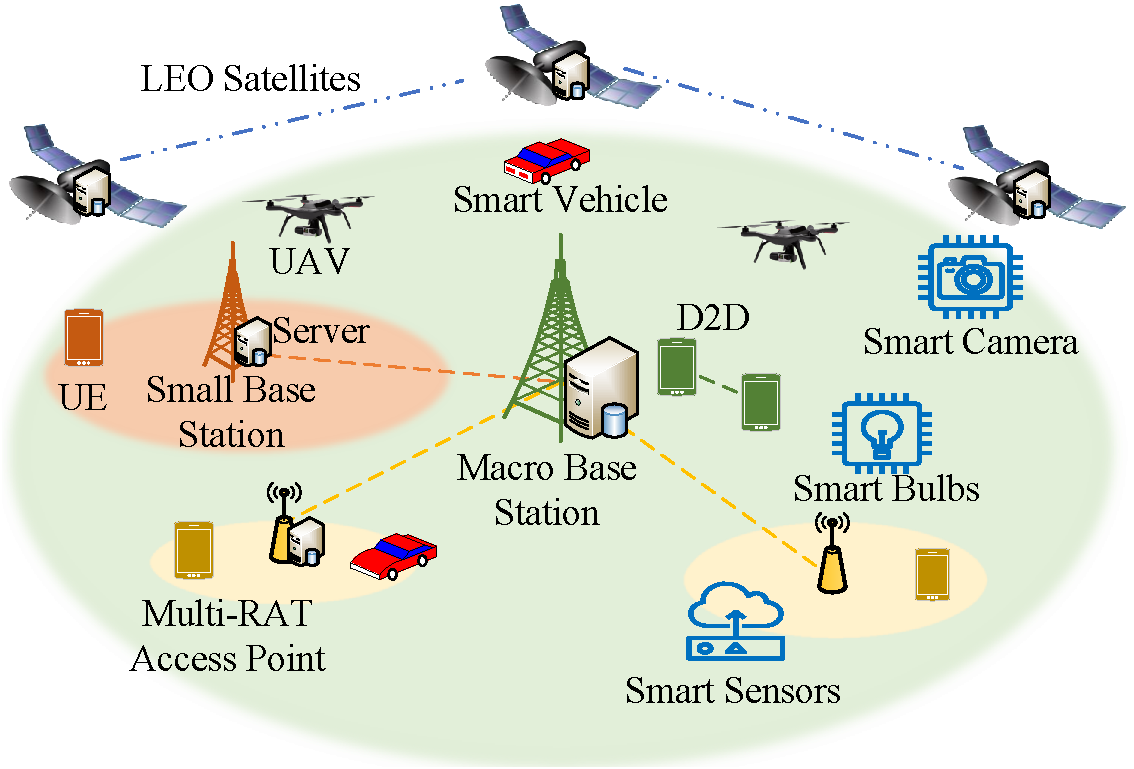
\includegraphics[width=0.9\columnwidth]{figures/SAGIN.pdf}
\caption{Correctness-aware monitoring over a satellite-ground integrated network under satellite disruption.}
\label{Fig1}
\end{figure}

We consider a satellite-ground integrated edge network in which monitoring edge nodes (UEs) observe time-varying
physical processes and transmit status updates to edge servers hosted at terrestrial base stations (BSs) or at
visible low-earth-orbit satellites (SATs). Let $\mathscr{U}$, $\mathscr{S}$, and $\mathscr{B}$ denote the sets of UEs,
SATs, and BSs, indexed by $u_i$, $s_j$, and $b_n$, and let $\mathscr{M}=\mathscr{S}\cup\mathscr{B}$ be the set of
serving nodes. Each serving node hosts an edge server that keeps a running estimate of every process assigned to it
and acts on that estimate. Time is slotted with slot duration $T_s$. UEs have low mobility over a decision interval;
the satellite topology changes continuously because of orbital motion. Table~\ref{tab:notation} lists the notation.

In contrast to the task-offloading models that dominate SAGIN edge computing, the quantity of interest here is the
correctness of the server's estimate. It depends on the dynamics of the monitored process, on when the UE samples and
transmits, and on whether the transmission is delivered before the process moves again. Satellite handover and
shadowing make the last of these uncertain, and an allocation chosen under nominal channel conditions can leave the
server with an estimate that is wrong rather than late.

The network is partitioned into $K$ local satellite-ground domains $\mathcal{D}_k=(\mathscr{U}_k,\mathscr{S}_k,
\mathscr{B}_k)$, $k\in\mathscr{K}=\{1,\ldots,K\}$, where the UE subsets partition $\mathscr{U}$ and a SAT may be
visible to several domains. Each domain has a classical controller that builds and solves a local robust binary
problem with a hybrid QAOA solver; a classical coordinator reconciles the bandwidth of SATs shared across domains and
certifies every assembled network schedule by its exact worst-case AoII.

\begin{table}[!t]
\centering
\caption{Key Notations}
\label{tab:notation}
\footnotesize
\renewcommand{\arraystretch}{1.15}
\begin{tabular}{|p{0.27\columnwidth}|p{0.61\columnwidth}|}
\hline
\textbf{Symbol} & \textbf{Definition} \\
\hline
$\mathscr{U}$, $\mathscr{S}$, $\mathscr{B}$ & Sets of UEs, SATs, and BSs \\
\hline
$\mathscr{M}=\mathscr{S}\cup\mathscr{B}$ & Set of serving nodes \\
\hline
$\mathscr{K}$, $\mathcal{D}_k$ & Set of domains; $k$-th domain \\
\hline
$\alpha_{ij}$, $\omega_{in}$ & Association of $u_i$ with $s_j$, $b_n$ \\
\hline
$\beta^{us}_{ij}$, $\beta^{ub}_{in}$ & Bandwidth allocated to $u_i$ by $s_j$, $b_n$ \\
\hline
$B^{s}_{j}$, $B^{b}_{n}$ & Bandwidth capacity of $s_j$, $b_n$ \\
\hline
$R^{us}_{ij}(\ell)$, $R^{ub}_{in}$ & Uplink rate of $u_i$ to $s_j$ (scenario $\ell$), to $b_n$ \\
\hline
$V_{ij}(t)$, $\Theta$ & Elevation of $s_j$ at $u_i$; minimum elevation \\
\hline
$G^{u}$, $G^{s}$, $G^{b}$ & Antenna gains of the UE, SAT, and BS \\
\hline
$\lambda^{\mathrm{cl}}$, $\sigma_{\mathrm{sf}}$ & TR 38.811 clutter loss; shadow-fading deviation \\
\hline
$\mathscr{L}$, $\Omega$ & Scenario set ($L$ scenarios); uncertainty set \\
\hline
$T^{\mathrm{dis}}(\ell)$, $\tau_{imq}(\ell)$ & Disruption window; induced outage (slots) \\
\hline
$T_s$, $D_i$ & Slot duration; status-update size (bits) \\
\hline
$X_i(t)$, $\hat{X}_i(t)$ & Monitored source of $u_i$; edge estimate \\
\hline
$\mathcal{X}_i$, $P_i$, $\pi_i$ & State space, transition matrix, stationary distribution \\
\hline
$f_i(x,\hat{x})$ & Distortion function \\
\hline
$\Delta_i^{II}(t)$, $\Delta_i^{II,\max}$ & Instantaneous AoII; AoII budget \\
\hline
$t_{i,\kappa}$, $Y_{i,\kappa}$ & $\kappa$-th delivery slot; inter-delivery interval \\
\hline
$\Psi_i(Y)$ & Expected AoII accumulated over an interval of length $Y$ \\
\hline
$\rho_i$, $\bar\rho_i^{h}$ & Update rate of $u_i$; $h$-th rate level ($H_i$ levels) \\
\hline
$\bar\beta_m^{q}$ & $q$-th bandwidth level of node $m$ ($Q_m$ levels) \\
\hline
$x_{imqh}$ & $1$ if $u_i$ uses node $m$, bandwidth level $q$, rate level $h$ \\
\hline
$\mathscr{A}_i$, $\mathscr{C}_i$ & Admissible combinations of $u_i$; pruned candidates \\
\hline
$\psi^{(\ell)}_{imqh}$ & Time-average AoII cost under scenario $\ell$ \\
\hline
$\mathbf{w}$, $\eta$ & Scenario weights; worst-case AoII (epigraph) \\
\hline
$T^{\mathrm{f}}$, $T^{\mathrm{b}}$ & Failure-detection window; blocking duration (slots) \\
\hline
$z_{jk}$, $u_{jk}$, $\varrho$ & ADMM bandwidth target, scaled dual, penalty \\
\hline
\end{tabular}
\end{table}

\subsection{Satellite Geometry and Communications Model}

Satellite positions are obtained from a constellation ephemeris. In the evaluation we propagate a public two-line
element set with SGP4~\cite{Vallado2006}, but the model only requires, for every SAT $s_j$ and UE $u_i$, the slant
range $d^{us}_{ij}(t)$ and the elevation angle $V_{ij}(t)$ in each slot. A SAT can serve $u_i$ in slot $t$ only if
$V_{ij}(t)\geq\Theta$. Each UE is served by the SAT that it has been handed to and keeps that SAT until it sets below
$\Theta$, at which point the UE is handed over to the SAT with the highest elevation; a dense constellation therefore
produces a sequence of passes of several minutes each, separated by handover interruptions, and no coverage gaps at
the elevation masks considered here.

The nominal path loss (in dB) between $u_i$ and $s_j$ is
\begin{equation}
    \varphi^{us}_{ij}=\varsigma^{us}+\zeta^{us}\log_{10}\!\left(f_{c}^{us}\right)
    +\xi^{us}\log_{10}\!\left(d^{us}_{ij}\right)+\lambda^{\mathrm{atm}}(V_{ij}),
\end{equation}
where $f_c^{us}$ is the carrier frequency, $\varsigma^{us}$, $\zeta^{us}$, and $\xi^{us}$ are the reference loss and
the frequency and distance exponents of free-space propagation, and $\lambda^{\mathrm{atm}}(V)$ is the atmospheric
absorption, which scales with $1/\sin V$. The UE-BS path loss $\varphi^{ub}_{in}$ uses the ground distance $d^{ub}_{in}$
and a terrestrial exponent $\xi^{ub}>2$ with a fixed margin. The received power at the SAT is
$p_i+G^{u}+G^{s}-\varphi^{us}_{ij}$ in dBm, where $p_i$ is the UE transmit power and $G^{u}$ and $G^{s}$ are the
antenna gains of the UE terminal and the satellite; the BS link uses $G^{b}$ in place of $G^{s}$ and the UE's sub-6-GHz
gain. The nominal uplink rate from $u_i$ to $s_j$ with bandwidth $\beta^{us}_{ij}$ is
\begin{equation}
    R^{us}_{ij}=\beta_{ij}^{us}\,\min\!\left\{\log_{2}\!\left(1+
    \frac{10^{(p_{i}+G^{u}+G^{s}-\varphi^{us}_{ij})/10}}{N_0\,\beta^{us}_{ij}\,F^{s}}\right),\ \bar{\gamma}\right\},
    \label{eq:rate_us}
\end{equation}
where $N_0$ is the noise power spectral density, $F^{s}$ the receiver noise figure, and $\bar\gamma$ the spectral
efficiency of the highest modulation and coding scheme. The UE-BS rate $R^{ub}_{in}$ is defined in the same way. Each
serving node divides its bandwidth among the UEs it serves, so the rate of a link does not depend on the association
decisions of other UEs once the bandwidth level is fixed. We treat co-channel interference as absorbed in the noise
figure and do not model residual Doppler, which the NTN frequency pre-compensation removes to within the subcarrier
spacing.

\emph{Large-scale channel.} On top of the nominal loss, each satellite link carries a large-scale state drawn once per
pass from the TR 38.811 model~\cite{TR38811}: with the elevation-dependent probability $p_{\mathrm{LOS}}(V)$ of the
chosen environment the pass is in line of sight; otherwise it is in non-line-of-sight and carries the clutter loss
$\lambda^{\mathrm{cl}}(V)$ of the carrier band, which at Ku band and suburban elevations is 17 to 25 dB. A shadow-fading
term with the state-dependent standard deviation $\sigma_{\mathrm{sf}}(V)$ is drawn per pass, and a small-scale fading
term per slot. In the suburban environment used in Section~VI roughly one pass segment in twenty is in
non-line-of-sight, and such a pass blocks the link for its whole duration at any bandwidth level.

\subsection{Monitored Source and Estimation Model}

Each UE $u_i$ observes a process $X_i(t)$ modeled as a discrete-time Markov chain on a finite state space
$\mathcal{X}_i$ with transition matrix $P_i$, in which the states are ordered severity or status levels. The UE
controls a generation indicator $g_i(t)\in\{0,1\}$ that specifies whether an update is sampled and transmitted in
slot $t$. We assume that $T_s$ exceeds the transmission and propagation delay of a successful update, so that an update
sampled at the start of slot $t$ is delivered within that slot or lost. Let $t_{i,\kappa}$ be the $\kappa$-th slot in
which an update from $u_i$ is delivered and $Y_{i,\kappa}=t_{i,\kappa+1}-t_{i,\kappa}$ the inter-delivery interval.
The server assigned to $u_i$ holds the estimate
\begin{equation}
    \hat{X}_i(t)=X_i(t_{i,\kappa}),\qquad t_{i,\kappa}\leq t<t_{i,\kappa+1},
\end{equation}
which is fixed between deliveries while the process keeps moving. With $\Lambda_i(t)=\max\{\tau\leq t:
X_i(\tau)=\hat{X}_i(\tau)\}$ the most recent slot in which the estimate was correct, the instantaneous AoII
is~\cite{Maatouk2020}
\begin{equation}
    \Delta_i^{II}(t)=\bigl(t-\Lambda_i(t)\bigr)\,f_i\!\left(X_i(t),\hat{X}_i(t)\right),
    \label{eq:aoii_def}
\end{equation}
where $f_i(x,\hat{x})\geq 0$ with $f_i(x,x)=0$ measures the severity of a mismatch; we use $f_i(x,\hat{x})=|x-\hat{x}|$.
AoII returns to zero without a delivery whenever the process revisits the estimated state, and becomes positive right
after a delivery if the process leaves the delivered state.

\subsection{Disruption Scenarios}

The orchestrator plans against a finite scenario set $\mathscr{L}=\{1,\ldots,L\}$, each scenario $\ell$ specifying an
additional loss $\delta^{us}_{ij}(\ell)$ on every UE-SAT link and a window length $T^{\mathrm{dis}}(\ell)$, in slots,
over which it applies:
\begin{equation}
    \tilde{\varphi}^{us}_{ij}(\ell)=\varphi^{us}_{ij}+\delta^{us}_{ij}(\ell).
    \label{eq:realized_pathloss}
\end{equation}
The scenario rate $R^{us}_{ij}(\ell)$ follows from~\eqref{eq:rate_us} with $\tilde{\varphi}^{us}_{ij}(\ell)$ in place
of $\varphi^{us}_{ij}$, and an update sampled in slot $t$ is delivered under scenario $\ell$ only if
$R^{us}_{ij}(\ell)\,T_s\geq D_i$ and $V_{ij}(t)\geq\Theta$, where $D_i$ is the size of an update in bits. BS links are
terrestrial and unaffected.

We use five scenarios. The first is the nominal channel. The second is a deep shadowing event in which every
satellite link loses $\sigma_{\mathrm{sf}}$ of the non-line-of-sight state, 12 dB in the suburban tables, for a window
of $T^{\mathrm{dis}}$ slots; it stands for the shadow fading of a pass that enters non-line-of-sight. The third and
fourth are the handover interruption of each individual satellite, a complete outage of that link for the duration
of a handover; and the fifth is the joint outage of all satellites for the deep-shadowing window, the global worst
case. An earlier version of the set also contained a mild 6 dB shadowing scenario. The sensitivity study of
Section~VI shows that it never binds: with the antenna gains of Table~I the satellite links keep a margin above the
delivery threshold at 6 dB, so no schedule changes when that scenario is added or removed, and we omit it. The study
also shows that the certified worst case and the hedging behaviour of the robust schedule appear only once the
handover of the second shared satellite is in the set, which is why the handover scenarios are kept per satellite
rather than merged.

In an offloading model a scenario perturbs the rate. Here it also determines the length of the outage window and
therefore the inter-delivery interval $Y_{i,\kappa}(\ell)$, the number of slots from $t_{i,\kappa}$ until the next slot
in which $g_i(t)=1$ and the delivery condition holds. A longer window lets $X_i(t)$ pass through more states before
the next delivery. The scenario set is the planner's model of the disruption process; the simulator of Section~VI
draws its disruptions from the TR 38.811 state process and the ephemeris, and the agreement between the two is what
the certificate's validity measures.

\subsection{Renewal-Interval AoII Decomposition}

Because $\Delta_i^{II}(t)$ depends on the trajectory of $X_i(t)$ since the estimate was last correct, it is not a
per-slot function of the channel state and cannot be used directly as the cost coefficient of a binary variable. The
delivery process is, however, a renewal process. Under the same-slot delivery assumption the estimate is exact at each
delivery, so $\Delta_i^{II}(t_{i,\kappa})=0$, and between two deliveries the estimate is fixed at
$\hat{x}=X_i(t_{i,\kappa})$ while the AoII evolves under the source's own dynamics, independently of the channel.

Let $\tilde{P}_{i,\hat{x}}=P_i\bigl(\mathbf{I}-\mathbf{e}_{\hat{x}}\mathbf{e}_{\hat{x}}^{\top}\bigr)$ be the taboo
matrix with the $\hat{x}$-th column of $P_i$ set to zero, so that $[\tilde{P}_{i,\hat{x}}^{a}]_{\hat{x}y}$ is the
probability of moving from $\hat{x}$ to $y$ in $a$ steps without returning to $\hat{x}$, and let
$\mathbf{f}_{i,\hat{x}}$ be the vector with entries $f_i(y,\hat{x})$. The AoII $s$ slots after a delivery equals
$a\,f_i(y,\hat{x})$ exactly when the source was last at $\hat{x}$ at slot $s-a$ and has since moved to $y$ without
returning, so
\begin{equation}
    \mathbb{E}\!\left[\Delta_i^{II}(t_{i,\kappa}+s)\,\middle|\,\hat{x}\right]
    =\sum_{a=1}^{s} a\,\bigl[P_i^{\,s-a}\bigr]_{\hat{x}\hat{x}}
    \bigl[\tilde{P}_{i,\hat{x}}^{\,a}\,\mathbf{f}_{i,\hat{x}}\bigr]_{\hat{x}},
    \label{eq:aoii_slot}
\end{equation}
and the expected AoII accumulated over an interval of length $Y$ is
\begin{align}
    \Psi_i(Y\mid\hat{x})&=\sum_{s=1}^{Y-1}
    \mathbb{E}\!\left[\Delta_i^{II}(t_{i,\kappa}+s)\,\middle|\,\hat{x}\right],
    \nonumber\\
    \Psi_i(Y)&=\sum_{\hat{x}\in\mathcal{X}_i}\pi_i(\hat{x})\,\Psi_i(Y\mid\hat{x}),
    \label{eq:psi_def}
\end{align}
where $\pi_i$ is the stationary distribution of $P_i$. Averaging over $\pi_i$ is legitimate because the update
decisions do not depend on the realized source state, so the delivered state is stationary. By the renewal-reward
theorem the time-average AoII of $u_i$ when its deliveries are $Y$ slots apart is $\Psi_i(Y)/Y$. Both quantities depend
only on $Y$ and $P_i$ and are tabulated once per UE for $Y\leq Y^{\max}$; we verified the table against Monte Carlo
simulation of the source and delivery process over $1.5\times 10^{6}$ slots, with agreement within one percent at every
interval length used.

Equation~\eqref{eq:psi_def} separates the source from the channel. The only channel-dependent quantity the planner
must reason about is the inter-delivery interval, which under scenario $\ell$ is deterministic for a given allocation
and is denoted $Y_i(\ell)$; the cost is the tabulated ratio $\Psi_i(Y_i(\ell))/Y_i(\ell)$.

\subsection{Binary Decision Model}

The update rates and bandwidths are continuous. We discretize the bandwidth of each node $m\in\mathscr{M}$ into $Q_m$
levels $\{\bar\beta_m^1,\ldots,\bar\beta_m^{Q_m}\}$ and the update rate of $u_i$ into $H_i$ levels
$\{\bar\rho_i^1,\ldots,\bar\rho_i^{H_i}\}\subset[\rho_i^{\min},\rho_i^{\max}]$, and define
\begin{equation}
    x_{imqh}=
    \begin{cases}
        1, & \text{if } u_i \text{ uses node } m\text{, level } q\text{, rate } h, \\
        0, & \text{otherwise}.
    \end{cases}
    \label{eq:x_def}
\end{equation}
The original decisions are recovered as $\alpha_{ij}=\sum_{q,h}x_{ijqh}$, $\omega_{in}=\sum_{q,h}x_{inqh}$,
$\beta^{us}_{ij}=\sum_{q,h}\bar\beta_j^q\,x_{ijqh}$, $\beta^{ub}_{in}=\sum_{q,h}\bar\beta_n^q\,x_{inqh}$, and
$\rho_i=\sum_{m,q,h}\bar\rho_i^h\,x_{imqh}$. The scenario does not index the variable, because it is realized by the
environment rather than chosen; each variable instead carries $L$ precomputed cost coefficients. After the
inadmissible combinations are removed (Section~IV-A) the number of decision variables is
\begin{equation}
    N_{x}=\sum_{i\in\mathscr{U}}|\mathscr{A}_i|\;\leq\;\sum_{i\in\mathscr{U}}\sum_{m\in\mathscr{M}}Q_{m}H_{i},
    \label{eq:Nx}
\end{equation}
which grows linearly with the number of UEs, nodes, and levels. Section~V prunes each $\mathscr{A}_i$ further to a
candidate set $\mathscr{C}_i$ of the $\kappa$ combinations with the smallest worst-case cost, which in our instances
never changed the optimum and reduced the qubit count by a further factor of two to three.

\subsection{Delivery Feedback and Link-Failure Handling}

A serving node acknowledges each delivered update, so a UE knows at the end of a slot whether its transmission
succeeded. A UE whose transmissions to a node have failed in every slot of a window of $T^{\mathrm{f}}$ slots declares
the link failed and avoids that node for $T^{\mathrm{b}}$ slots or, for a satellite, until its next handover; its
controller is informed and re-solves the domain problem without the failed link at the next orchestration interval.
This rule is applied uniformly to every policy in Section~VI, because any state-aware baseline needs the same
information to be competitive, and because the value of a robust schedule depends on whether such feedback exists.
Both regimes are reported.

\subsection{Distributed Orchestration Model}

Each domain $\mathcal{D}_k$ holds the local decision vector $\mathbf{x}_k=\{x_{imqh}\mid u_i\in\mathscr{U}_k,\,
(m,q,h)\in\mathscr{C}_i\}$ and the local state $\mathbf{s}_k=[\boldsymbol{\Psi}_k,\mathbf{V}_k,\mathbf{X}_k,
\mathbf{B}_k,\mathbf{E}_k,\boldsymbol{\Xi}_k]$, with $\boldsymbol{\Psi}_k$ the tabulated AoII costs of its UEs,
$\mathbf{V}_k$ the elevations, $\mathbf{X}_k$ the transition matrices and budgets, $\mathbf{B}_k$ the bandwidth levels,
$\mathbf{E}_k$ the ephemeris over the decision interval, and $\boldsymbol{\Xi}_k$ the scenario set restricted to the
domain. The controller re-solves its problem whenever a satellite becomes visible or sets, when a link failure is
reported, and in any case at a fixed re-solve period. Within one solve, a classical outer loop maintains scenario
weights, each domain solves a linear assignment subproblem on a quantum sampler, and the coordinator runs the sharing
form of ADMM on the bandwidth of shared satellites and evaluates the worst-case AoII of each assembled schedule
exactly. The orchestration latency, the time from the start of a solve until its schedule is in force, extends every
inter-delivery interval by $\epsilon_i$ slots and enters the cost through $\Psi_i(Y_i(\ell)+\epsilon_i)$; in the
evaluation the solve time is measured and reported rather than assumed.

%=======================================================================
\section{Problem Formulation}
%=======================================================================

The objective is to minimize the worst-case time-average AoII across all monitored UEs over the scenario set, by
jointly choosing update rates, association, and bandwidth. Let $\boldsymbol{\chi}_i=\bigl(\rho_i,\{\alpha_{ij}\}_{j},
\{\omega_{in}\}_{n},\{\beta^{us}_{ij}\}_{j},\{\beta^{ub}_{in}\}_{n}\bigr)$ collect the decisions of $u_i$ and
$Y_i(\boldsymbol{\chi}_i,\boldsymbol{\xi})$ its inter-delivery interval under realization $\boldsymbol{\xi}\in\Omega$.
The robust Value-of-information-aware, uncertainty-robust, Network-wide Generation, Update-scheduling, Association,
and Resource orchestration under Disruption (VANGUARD) problem is
\begin{align}
    \mathscr{P}_{1}:\;&\min_{\{\boldsymbol{\chi}_i\}_{i\in\mathscr{U}}}
    \;\max_{\boldsymbol{\xi}\in\Omega}
    \;\frac{1}{|\mathscr{U}|}\sum_{i\in\mathscr{U}}
    \frac{\Psi_{i}\bigl(Y_{i}(\boldsymbol{\chi}_i,\boldsymbol{\xi})\bigr)}
    {Y_{i}(\boldsymbol{\chi}_i,\boldsymbol{\xi})}
    \nonumber\\
    \text{s.t.}\;\;
    &\text{C1}:\sum_{j\in\mathscr{S}}\alpha_{ij}+\sum_{n\in\mathscr{B}}\omega_{in}=1,\;\forall\,i\in\mathscr{U},
    \nonumber\\
    &\text{C2}:\sum_{i\in\mathscr{U}}\alpha_{ij}\,\beta^{us}_{ij}\leq B^{s}_{j},\;\forall\,j\in\mathscr{S},
    \nonumber\\
    &\text{C3}:\sum_{i\in\mathscr{U}}\omega_{in}\,\beta^{ub}_{in}\leq B^{b}_{n},\;\forall\,n\in\mathscr{B},
    \nonumber\\
    &\text{C4}:\frac{\Psi_{i}\bigl(Y_{i}(\boldsymbol{\chi}_i,\boldsymbol{\xi})\bigr)}
    {Y_{i}(\boldsymbol{\chi}_i,\boldsymbol{\xi})}\leq\Delta_{i}^{II,\max},
    \;\forall\,i\in\mathscr{U},\;\forall\,\boldsymbol{\xi}\in\Omega,
    \nonumber\\
    &\text{C5}:\alpha_{ij}\bigl(V_{ij}-\Theta\bigr)\geq 0,\;\forall\,i\in\mathscr{U},\;\forall\,j\in\mathscr{S},
    \nonumber\\
    &\text{C6}:\rho_{i}^{\min}\leq\rho_{i}\leq\rho_{i}^{\max},\;\forall\,i\in\mathscr{U},
    \nonumber\\
    &\text{C7}:\alpha_{ij},\,\omega_{in}\in\{0,1\},\;\forall\,i,j,n.
    \nonumber
\end{align}
C1 routes each UE through exactly one serving node per decision interval. C2 and C3 are the bandwidth capacities. C4
is the correctness constraint: the expected time-average AoII of every UE stays within its budget
$\Delta_i^{II,\max}$ under every realization, including the worst. It is stated in expectation because the
instantaneous AoII of a Markov source cannot be bounded deterministically; the source may stay in a mismatched state
for a whole interval. C5 restricts association to visible satellites, C6 bounds the update rate by the freshness
requirement and the UE's energy or channel-access budget, and C7 makes association binary.

$\mathscr{P}_{1}$ is a mixed-integer nonlinear minimax program. With a single scenario and fixed rates it contains the
generalized assignment problem and is NP-hard. The inner maximization adds a difficulty of its own: because $\Psi_i$
is a nonlinear, source-specific function of the interval, the realization that maximizes the network AoII is not
necessarily the one with the worst channel, since it also depends on how the volatility of each source interacts with
the outage that the realization induces. The feasible association set defined by C5 changes at every decision
interval as satellites move.

\subsection{Robust Binary Reformulation}

With the discretization of Section~III-E and the variable $x_{imqh}$ of~\eqref{eq:x_def}, each scenario $\ell$ gives,
for every UE-node pair and bandwidth level, a rate $R_{imq}(\ell)$ from~\eqref{eq:rate_us} with the scenario path
loss. The link is in outage throughout the scenario window if that rate cannot deliver an update within a slot, so the
induced outage is
\begin{equation}
    \tau_{imq}(\ell)=
    \begin{cases}
        T^{\mathrm{dis}}(\ell)\,\mathbb{I}\bigl\{R_{imq}(\ell)\,T_s<D_i\bigr\}, & m\in\mathscr{S},\\
        0, & m\in\mathscr{B}.
    \end{cases}
    \label{eq:tau_out}
\end{equation}
The bandwidth level matters: a larger allocation can keep the rate above the delivery threshold through deep
shadowing, whereas a handover interruption is an outage at any bandwidth. A UE whose update fails during an outage
transmits a fresh sample as soon as the link returns. The worst case is an outage that begins at a scheduled sampling
slot, which gives
\begin{equation}
    Y_{imqh}(\ell)=\left\lceil\frac{1}{\bar\rho_i^{h}T_s}\right\rceil+\tau_{imq}(\ell),\qquad
    \psi_{imqh}^{(\ell)}=\frac{\Psi_{i}\bigl(Y_{imqh}(\ell)\bigr)}{Y_{imqh}(\ell)},
    \label{eq:psi_imqh}
\end{equation}
precomputed for every $(i,m,q,h,\ell)$; with orchestration overhead, $Y_{imqh}(\ell)+\epsilon_i$ replaces
$Y_{imqh}(\ell)$.

\emph{Pre-elimination.} The admissible set $\mathscr{A}_i$ consists of the combinations $(m,q,h)$ for which (i)
$m\in\mathscr{B}$, or $m\in\mathscr{S}$ with $V_{im}\geq\Theta$; (ii) the nominal rate satisfies
$R_{imq}T_s\geq D_i$; and (iii) $\max_{\ell}\psi^{(\ell)}_{imqh}\leq\Delta_i^{II,\max}$. Condition (i) enforces C5
and (iii) is the discrete form of C4. Since each UE selects exactly one combination, it meets its budget under every
scenario if and only if its selection lies in $\mathscr{A}_i$; the budget is thus enforced by removing variables
rather than by adding penalty terms, which costs no qubits. A UE for which $\mathscr{A}_i$ is empty, which happens for
a satellite-only UE whose budget is below the AoII of a full handover outage, is assigned its least-bad combination and
reported as a budget violation; Section~VI states how often this occurs.

The binary reformulation of VANGUARD is
\begin{align}
    \mathscr{P}_{2}:\;&\min_{\mathbf{x}}\;\max_{\ell\in\mathscr{L}}\;
    \frac{1}{|\mathscr{U}|}\sum_{i\in\mathscr{U}}\sum_{(m,q,h)\in\mathscr{A}_i}\psi_{imqh}^{(\ell)}\,x_{imqh}
    \nonumber\\
    \text{s.t.}\;\;
    &\text{D1}:\sum_{(m,q,h)\in\mathscr{A}_i}x_{imqh}=1,\;\forall\,i\in\mathscr{U},
    \nonumber\\
    &\text{D2}:\sum_{i\in\mathscr{U}}\sum_{(j,q,h)\in\mathscr{A}_i}\bar{\beta}^{q}_{j}\,x_{ijqh}\leq B^{s}_{j},
    \;\forall\,j\in\mathscr{S},
    \nonumber\\
    &\text{D3}:\sum_{i\in\mathscr{U}}\sum_{(n,q,h)\in\mathscr{A}_i}\bar{\beta}^{q}_{n}\,x_{inqh}\leq B^{b}_{n},
    \;\forall\,n\in\mathscr{B},
    \nonumber\\
    &\text{D4}:x_{imqh}\in\{0,1\},\;\forall\,i\in\mathscr{U},\;(m,q,h)\in\mathscr{A}_i.
    \nonumber
\end{align}
D1 is the one-hot selection, D2 and D3 the discrete capacities, D4 the binary domain.

\subsection{Epigraph Form, Certificate, and Exact Reference}

Introducing the worst-case value $\eta$ gives the equivalent epigraph form
\begin{align}
    \mathscr{P}_{3}:\;&\min_{\mathbf{x},\,\eta}\;\eta
    \nonumber\\
    \text{s.t.}\;\;&\text{E1}:\frac{1}{|\mathscr{U}|}\sum_{i\in\mathscr{U}}\sum_{(m,q,h)\in\mathscr{A}_i}
    \psi_{imqh}^{(\ell)}\,x_{imqh}\leq\eta,\;\forall\,\ell\in\mathscr{L},
    \nonumber\\
    &\text{D1--D4},
    \nonumber
\end{align}
in which E1 is tight for at least one scenario at the optimum. $\mathscr{P}_{3}$ serves two purposes in this paper,
neither of which is to be solved on a quantum device. First, it is the certificate: for any schedule $\mathbf{x}$
returned by any solver, the $L$ left-hand sides of E1 are evaluated exactly, so the worst-case time-average AoII of
that schedule over $\mathscr{L}$ is known with certainty. Second, $\mathscr{P}_{3}$ is a mixed-integer linear program,
and up to 75 UEs it is solved to proven optimality by a branch-and-cut solver~\cite{HiGHS2018} in well under a
second, with a time limit reached only on some 100-UE instances; this gives an exact reference for every heuristic and
quantum solver we compare. A direct
QUBO encoding of $\mathscr{P}_{3}$, with $\eta$ on a binary grid and a slack register for each of the $L$
constraints E1, was the encoding of an earlier version of this work; it multiplies the qubit count by three to four
and produces a penalty landscape in which neither simulated annealing nor QAOA found a feasible assignment on
instances of ten UEs. Section~V therefore works with $\mathscr{P}_{2}$ directly, replacing the inner maximization by
scenario weights so that every quantum subproblem is linear in $\mathbf{x}$ and the only auxiliary qubits are the
slack bits of the capacity constraints D2 and D3.
